% Created by tikzDevice version 0.6.2-92-0ad2792 on 2013-04-07 18:00:37
% !TEX encoding = UTF-8 Unicode
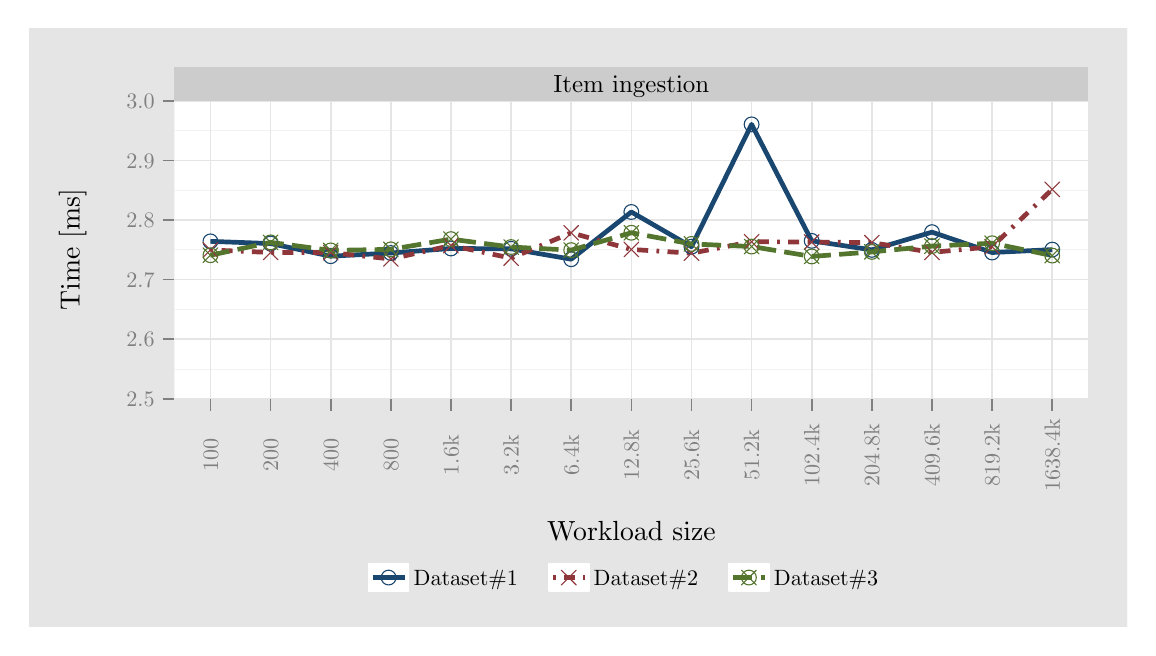
\begin{tikzpicture}[x=1pt,y=1pt]
\definecolor[named]{fillColor}{rgb}{1.00,1.00,1.00}
\path[use as bounding box,fill=fillColor,fill opacity=0.00] (0,0) rectangle (397.48,216.81);
\begin{scope}
\path[clip] (  0.00,  0.00) rectangle (397.48,216.81);
\definecolor[named]{drawColor}{rgb}{1.00,1.00,1.00}
\definecolor[named]{fillColor}{rgb}{0.90,0.90,0.90}

\path[draw=drawColor,line width= 0.6pt,line join=round,line cap=round,fill=fillColor] (  0.00,  0.00) rectangle (397.48,216.81);
\end{scope}
\begin{scope}
\path[clip] ( 53.00, 82.69) rectangle (383.26,190.36);
\definecolor[named]{fillColor}{rgb}{1.00,1.00,1.00}

\path[fill=fillColor] ( 53.00, 82.69) rectangle (383.26,190.36);
\definecolor[named]{drawColor}{rgb}{0.95,0.95,0.95}

\path[draw=drawColor,line width= 0.3pt,line join=round] ( 53.00, 93.46) --
	(383.26, 93.46);

\path[draw=drawColor,line width= 0.3pt,line join=round] ( 53.00,114.99) --
	(383.26,114.99);

\path[draw=drawColor,line width= 0.3pt,line join=round] ( 53.00,136.53) --
	(383.26,136.53);

\path[draw=drawColor,line width= 0.3pt,line join=round] ( 53.00,158.06) --
	(383.26,158.06);

\path[draw=drawColor,line width= 0.3pt,line join=round] ( 53.00,179.60) --
	(383.26,179.60);
\definecolor[named]{drawColor}{rgb}{0.90,0.90,0.90}

\path[draw=drawColor,line width= 0.6pt,line join=round] ( 53.00, 82.69) --
	(383.26, 82.69);

\path[draw=drawColor,line width= 0.6pt,line join=round] ( 53.00,104.23) --
	(383.26,104.23);

\path[draw=drawColor,line width= 0.6pt,line join=round] ( 53.00,125.76) --
	(383.26,125.76);

\path[draw=drawColor,line width= 0.6pt,line join=round] ( 53.00,147.29) --
	(383.26,147.29);

\path[draw=drawColor,line width= 0.6pt,line join=round] ( 53.00,168.83) --
	(383.26,168.83);

\path[draw=drawColor,line width= 0.6pt,line join=round] ( 53.00,190.36) --
	(383.26,190.36);

\path[draw=drawColor,line width= 0.6pt,line join=round] ( 66.04, 82.69) --
	( 66.04,190.36);

\path[draw=drawColor,line width= 0.6pt,line join=round] ( 87.77, 82.69) --
	( 87.77,190.36);

\path[draw=drawColor,line width= 0.6pt,line join=round] (109.50, 82.69) --
	(109.50,190.36);

\path[draw=drawColor,line width= 0.6pt,line join=round] (131.22, 82.69) --
	(131.22,190.36);

\path[draw=drawColor,line width= 0.6pt,line join=round] (152.95, 82.69) --
	(152.95,190.36);

\path[draw=drawColor,line width= 0.6pt,line join=round] (174.68, 82.69) --
	(174.68,190.36);

\path[draw=drawColor,line width= 0.6pt,line join=round] (196.40, 82.69) --
	(196.40,190.36);

\path[draw=drawColor,line width= 0.6pt,line join=round] (218.13, 82.69) --
	(218.13,190.36);

\path[draw=drawColor,line width= 0.6pt,line join=round] (239.86, 82.69) --
	(239.86,190.36);

\path[draw=drawColor,line width= 0.6pt,line join=round] (261.59, 82.69) --
	(261.59,190.36);

\path[draw=drawColor,line width= 0.6pt,line join=round] (283.31, 82.69) --
	(283.31,190.36);

\path[draw=drawColor,line width= 0.6pt,line join=round] (305.04, 82.69) --
	(305.04,190.36);

\path[draw=drawColor,line width= 0.6pt,line join=round] (326.77, 82.69) --
	(326.77,190.36);

\path[draw=drawColor,line width= 0.6pt,line join=round] (348.50, 82.69) --
	(348.50,190.36);

\path[draw=drawColor,line width= 0.6pt,line join=round] (370.22, 82.69) --
	(370.22,190.36);
\definecolor[named]{drawColor}{rgb}{0.10,0.28,0.44}

\path[draw=drawColor,line width= 1.7pt,line join=round] ( 66.04,139.59) --
	( 87.77,138.80) --
	(109.50,134.23) --
	(131.22,135.39) --
	(152.95,137.02) --
	(174.68,136.91) --
	(196.40,133.14) --
	(218.13,150.21) --
	(239.86,137.65) --
	(261.59,181.86) --
	(283.31,139.77) --
	(305.04,136.51) --
	(326.77,142.92) --
	(348.50,135.56) --
	(370.22,136.61);
\definecolor[named]{drawColor}{rgb}{0.56,0.21,0.23}

\path[draw=drawColor,line width= 1.7pt,dash pattern=on 1pt off 3pt on 4pt off 3pt ,line join=round] ( 66.04,136.47) --
	( 87.77,135.58) --
	(109.50,135.53) --
	(131.22,133.23) --
	(152.95,138.09) --
	(174.68,133.53) --
	(196.40,142.68) --
	(218.13,136.67) --
	(239.86,135.32) --
	(261.59,139.45) --
	(283.31,139.35) --
	(305.04,139.14) --
	(326.77,135.60) --
	(348.50,137.67) --
	(370.22,158.40);
\definecolor[named]{drawColor}{rgb}{0.33,0.46,0.18}

\path[draw=drawColor,line width= 1.7pt,dash pattern=on 7pt off 3pt ,line join=round] ( 66.04,134.58) --
	( 87.77,139.23) --
	(109.50,136.32) --
	(131.22,136.70) --
	(152.95,140.40) --
	(174.68,137.54) --
	(196.40,136.42) --
	(218.13,142.70) --
	(239.86,138.66) --
	(261.59,137.72) --
	(283.31,134.14) --
	(305.04,135.79) --
	(326.77,137.88) --
	(348.50,138.91) --
	(370.22,134.46);
\definecolor[named]{drawColor}{rgb}{0.10,0.28,0.44}

\path[draw=drawColor,line width= 0.4pt,line join=round,line cap=round] ( 66.04,139.59) circle (  2.67);

\path[draw=drawColor,line width= 0.4pt,line join=round,line cap=round] ( 87.77,138.80) circle (  2.67);

\path[draw=drawColor,line width= 0.4pt,line join=round,line cap=round] (109.50,134.23) circle (  2.67);

\path[draw=drawColor,line width= 0.4pt,line join=round,line cap=round] (131.22,135.39) circle (  2.67);

\path[draw=drawColor,line width= 0.4pt,line join=round,line cap=round] (152.95,137.02) circle (  2.67);

\path[draw=drawColor,line width= 0.4pt,line join=round,line cap=round] (174.68,136.91) circle (  2.67);

\path[draw=drawColor,line width= 0.4pt,line join=round,line cap=round] (196.40,133.14) circle (  2.67);

\path[draw=drawColor,line width= 0.4pt,line join=round,line cap=round] (218.13,150.21) circle (  2.67);

\path[draw=drawColor,line width= 0.4pt,line join=round,line cap=round] (239.86,137.65) circle (  2.67);

\path[draw=drawColor,line width= 0.4pt,line join=round,line cap=round] (261.59,181.86) circle (  2.67);

\path[draw=drawColor,line width= 0.4pt,line join=round,line cap=round] (283.31,139.77) circle (  2.67);

\path[draw=drawColor,line width= 0.4pt,line join=round,line cap=round] (305.04,136.51) circle (  2.67);

\path[draw=drawColor,line width= 0.4pt,line join=round,line cap=round] (326.77,142.92) circle (  2.67);

\path[draw=drawColor,line width= 0.4pt,line join=round,line cap=round] (348.50,135.56) circle (  2.67);

\path[draw=drawColor,line width= 0.4pt,line join=round,line cap=round] (370.22,136.61) circle (  2.67);
\definecolor[named]{drawColor}{rgb}{0.56,0.21,0.23}

\path[draw=drawColor,line width= 0.4pt,line join=round,line cap=round,fill=fillColor] ( 63.37,133.81) -- ( 68.71,139.14);

\path[draw=drawColor,line width= 0.4pt,line join=round,line cap=round,fill=fillColor] ( 63.37,139.14) -- ( 68.71,133.81);

\path[draw=drawColor,line width= 0.4pt,line join=round,line cap=round,fill=fillColor] ( 85.10,132.91) -- ( 90.44,138.25);

\path[draw=drawColor,line width= 0.4pt,line join=round,line cap=round,fill=fillColor] ( 85.10,138.25) -- ( 90.44,132.91);

\path[draw=drawColor,line width= 0.4pt,line join=round,line cap=round,fill=fillColor] (106.83,132.86) -- (112.16,138.20);

\path[draw=drawColor,line width= 0.4pt,line join=round,line cap=round,fill=fillColor] (106.83,138.20) -- (112.16,132.86);

\path[draw=drawColor,line width= 0.4pt,line join=round,line cap=round,fill=fillColor] (128.56,130.56) -- (133.89,135.90);

\path[draw=drawColor,line width= 0.4pt,line join=round,line cap=round,fill=fillColor] (128.56,135.90) -- (133.89,130.56);

\path[draw=drawColor,line width= 0.4pt,line join=round,line cap=round,fill=fillColor] (150.28,135.42) -- (155.62,140.75);

\path[draw=drawColor,line width= 0.4pt,line join=round,line cap=round,fill=fillColor] (150.28,140.75) -- (155.62,135.42);

\path[draw=drawColor,line width= 0.4pt,line join=round,line cap=round,fill=fillColor] (172.01,130.86) -- (177.34,136.20);

\path[draw=drawColor,line width= 0.4pt,line join=round,line cap=round,fill=fillColor] (172.01,136.20) -- (177.34,130.86);

\path[draw=drawColor,line width= 0.4pt,line join=round,line cap=round,fill=fillColor] (193.74,140.01) -- (199.07,145.35);

\path[draw=drawColor,line width= 0.4pt,line join=round,line cap=round,fill=fillColor] (193.74,145.35) -- (199.07,140.01);

\path[draw=drawColor,line width= 0.4pt,line join=round,line cap=round,fill=fillColor] (215.46,134.00) -- (220.80,139.33);

\path[draw=drawColor,line width= 0.4pt,line join=round,line cap=round,fill=fillColor] (215.46,139.33) -- (220.80,134.00);

\path[draw=drawColor,line width= 0.4pt,line join=round,line cap=round,fill=fillColor] (237.19,132.65) -- (242.53,137.98);

\path[draw=drawColor,line width= 0.4pt,line join=round,line cap=round,fill=fillColor] (237.19,137.98) -- (242.53,132.65);

\path[draw=drawColor,line width= 0.4pt,line join=round,line cap=round,fill=fillColor] (258.92,136.79) -- (264.25,142.12);

\path[draw=drawColor,line width= 0.4pt,line join=round,line cap=round,fill=fillColor] (258.92,142.12) -- (264.25,136.79);

\path[draw=drawColor,line width= 0.4pt,line join=round,line cap=round,fill=fillColor] (280.65,136.68) -- (285.98,142.02);

\path[draw=drawColor,line width= 0.4pt,line join=round,line cap=round,fill=fillColor] (280.65,142.02) -- (285.98,136.68);

\path[draw=drawColor,line width= 0.4pt,line join=round,line cap=round,fill=fillColor] (302.37,136.47) -- (307.71,141.81);

\path[draw=drawColor,line width= 0.4pt,line join=round,line cap=round,fill=fillColor] (302.37,141.81) -- (307.71,136.47);

\path[draw=drawColor,line width= 0.4pt,line join=round,line cap=round,fill=fillColor] (324.10,132.93) -- (329.44,138.27);

\path[draw=drawColor,line width= 0.4pt,line join=round,line cap=round,fill=fillColor] (324.10,138.27) -- (329.44,132.93);

\path[draw=drawColor,line width= 0.4pt,line join=round,line cap=round,fill=fillColor] (345.83,135.00) -- (351.16,140.33);

\path[draw=drawColor,line width= 0.4pt,line join=round,line cap=round,fill=fillColor] (345.83,140.33) -- (351.16,135.00);

\path[draw=drawColor,line width= 0.4pt,line join=round,line cap=round,fill=fillColor] (367.55,155.73) -- (372.89,161.07);

\path[draw=drawColor,line width= 0.4pt,line join=round,line cap=round,fill=fillColor] (367.55,161.07) -- (372.89,155.73);
\definecolor[named]{drawColor}{rgb}{0.33,0.46,0.18}

\path[draw=drawColor,line width= 0.4pt,line join=round,line cap=round] ( 66.04,134.58) circle (  2.67);

\path[draw=drawColor,line width= 0.4pt,line join=round,line cap=round] ( 63.37,131.91) -- ( 68.71,137.25);

\path[draw=drawColor,line width= 0.4pt,line join=round,line cap=round] ( 63.37,137.25) -- ( 68.71,131.91);

\path[draw=drawColor,line width= 0.4pt,line join=round,line cap=round] ( 87.77,139.23) circle (  2.67);

\path[draw=drawColor,line width= 0.4pt,line join=round,line cap=round] ( 85.10,136.56) -- ( 90.44,141.89);

\path[draw=drawColor,line width= 0.4pt,line join=round,line cap=round] ( 85.10,141.89) -- ( 90.44,136.56);

\path[draw=drawColor,line width= 0.4pt,line join=round,line cap=round] (109.50,136.32) circle (  2.67);

\path[draw=drawColor,line width= 0.4pt,line join=round,line cap=round] (106.83,133.65) -- (112.16,138.98);

\path[draw=drawColor,line width= 0.4pt,line join=round,line cap=round] (106.83,138.98) -- (112.16,133.65);

\path[draw=drawColor,line width= 0.4pt,line join=round,line cap=round] (131.22,136.70) circle (  2.67);

\path[draw=drawColor,line width= 0.4pt,line join=round,line cap=round] (128.56,134.03) -- (133.89,139.37);

\path[draw=drawColor,line width= 0.4pt,line join=round,line cap=round] (128.56,139.37) -- (133.89,134.03);

\path[draw=drawColor,line width= 0.4pt,line join=round,line cap=round] (152.95,140.40) circle (  2.67);

\path[draw=drawColor,line width= 0.4pt,line join=round,line cap=round] (150.28,137.73) -- (155.62,143.07);

\path[draw=drawColor,line width= 0.4pt,line join=round,line cap=round] (150.28,143.07) -- (155.62,137.73);

\path[draw=drawColor,line width= 0.4pt,line join=round,line cap=round] (174.68,137.54) circle (  2.67);

\path[draw=drawColor,line width= 0.4pt,line join=round,line cap=round] (172.01,134.88) -- (177.34,140.21);

\path[draw=drawColor,line width= 0.4pt,line join=round,line cap=round] (172.01,140.21) -- (177.34,134.88);

\path[draw=drawColor,line width= 0.4pt,line join=round,line cap=round] (196.40,136.42) circle (  2.67);

\path[draw=drawColor,line width= 0.4pt,line join=round,line cap=round] (193.74,133.75) -- (199.07,139.09);

\path[draw=drawColor,line width= 0.4pt,line join=round,line cap=round] (193.74,139.09) -- (199.07,133.75);

\path[draw=drawColor,line width= 0.4pt,line join=round,line cap=round] (218.13,142.70) circle (  2.67);

\path[draw=drawColor,line width= 0.4pt,line join=round,line cap=round] (215.46,140.03) -- (220.80,145.36);

\path[draw=drawColor,line width= 0.4pt,line join=round,line cap=round] (215.46,145.36) -- (220.80,140.03);

\path[draw=drawColor,line width= 0.4pt,line join=round,line cap=round] (239.86,138.66) circle (  2.67);

\path[draw=drawColor,line width= 0.4pt,line join=round,line cap=round] (237.19,136.00) -- (242.53,141.33);

\path[draw=drawColor,line width= 0.4pt,line join=round,line cap=round] (237.19,141.33) -- (242.53,136.00);

\path[draw=drawColor,line width= 0.4pt,line join=round,line cap=round] (261.59,137.72) circle (  2.67);

\path[draw=drawColor,line width= 0.4pt,line join=round,line cap=round] (258.92,135.05) -- (264.25,140.39);

\path[draw=drawColor,line width= 0.4pt,line join=round,line cap=round] (258.92,140.39) -- (264.25,135.05);

\path[draw=drawColor,line width= 0.4pt,line join=round,line cap=round] (283.31,134.14) circle (  2.67);

\path[draw=drawColor,line width= 0.4pt,line join=round,line cap=round] (280.65,131.48) -- (285.98,136.81);

\path[draw=drawColor,line width= 0.4pt,line join=round,line cap=round] (280.65,136.81) -- (285.98,131.48);

\path[draw=drawColor,line width= 0.4pt,line join=round,line cap=round] (305.04,135.79) circle (  2.67);

\path[draw=drawColor,line width= 0.4pt,line join=round,line cap=round] (302.37,133.12) -- (307.71,138.46);

\path[draw=drawColor,line width= 0.4pt,line join=round,line cap=round] (302.37,138.46) -- (307.71,133.12);

\path[draw=drawColor,line width= 0.4pt,line join=round,line cap=round] (326.77,137.88) circle (  2.67);

\path[draw=drawColor,line width= 0.4pt,line join=round,line cap=round] (324.10,135.21) -- (329.44,140.54);

\path[draw=drawColor,line width= 0.4pt,line join=round,line cap=round] (324.10,140.54) -- (329.44,135.21);

\path[draw=drawColor,line width= 0.4pt,line join=round,line cap=round] (348.50,138.91) circle (  2.67);

\path[draw=drawColor,line width= 0.4pt,line join=round,line cap=round] (345.83,136.24) -- (351.16,141.58);

\path[draw=drawColor,line width= 0.4pt,line join=round,line cap=round] (345.83,141.58) -- (351.16,136.24);

\path[draw=drawColor,line width= 0.4pt,line join=round,line cap=round] (370.22,134.46) circle (  2.67);

\path[draw=drawColor,line width= 0.4pt,line join=round,line cap=round] (367.55,131.79) -- (372.89,137.13);

\path[draw=drawColor,line width= 0.4pt,line join=round,line cap=round] (367.55,137.13) -- (372.89,131.79);
\end{scope}
\begin{scope}
\path[clip] (  0.00,  0.00) rectangle (397.48,216.81);
\definecolor[named]{fillColor}{rgb}{0.80,0.80,0.80}

\path[fill=fillColor] ( 53.00,190.36) rectangle (383.26,202.58);
\definecolor[named]{drawColor}{rgb}{0.00,0.00,0.00}

\node[text=drawColor,anchor=base,inner sep=0pt, outer sep=0pt, scale=  0.90] at (218.13,193.37) {Item ingestion};
\end{scope}
\begin{scope}
\path[clip] (  0.00,  0.00) rectangle (397.48,216.81);
\definecolor[named]{drawColor}{rgb}{0.50,0.50,0.50}

\node[text=drawColor,anchor=base east,inner sep=0pt, outer sep=0pt, scale=  0.80] at ( 45.89, 79.94) {2.5};

\node[text=drawColor,anchor=base east,inner sep=0pt, outer sep=0pt, scale=  0.80] at ( 45.89,101.47) {2.6};

\node[text=drawColor,anchor=base east,inner sep=0pt, outer sep=0pt, scale=  0.80] at ( 45.89,123.00) {2.7};

\node[text=drawColor,anchor=base east,inner sep=0pt, outer sep=0pt, scale=  0.80] at ( 45.89,144.54) {2.8};

\node[text=drawColor,anchor=base east,inner sep=0pt, outer sep=0pt, scale=  0.80] at ( 45.89,166.07) {2.9};

\node[text=drawColor,anchor=base east,inner sep=0pt, outer sep=0pt, scale=  0.80] at ( 45.89,187.61) {3.0};
\end{scope}
\begin{scope}
\path[clip] (  0.00,  0.00) rectangle (397.48,216.81);
\definecolor[named]{drawColor}{rgb}{0.50,0.50,0.50}

\path[draw=drawColor,line width= 0.6pt,line join=round] ( 48.74, 82.69) --
	( 53.00, 82.69);

\path[draw=drawColor,line width= 0.6pt,line join=round] ( 48.74,104.23) --
	( 53.00,104.23);

\path[draw=drawColor,line width= 0.6pt,line join=round] ( 48.74,125.76) --
	( 53.00,125.76);

\path[draw=drawColor,line width= 0.6pt,line join=round] ( 48.74,147.29) --
	( 53.00,147.29);

\path[draw=drawColor,line width= 0.6pt,line join=round] ( 48.74,168.83) --
	( 53.00,168.83);

\path[draw=drawColor,line width= 0.6pt,line join=round] ( 48.74,190.36) --
	( 53.00,190.36);
\end{scope}
\begin{scope}
\path[clip] (  0.00,  0.00) rectangle (397.48,216.81);
\definecolor[named]{drawColor}{rgb}{0.50,0.50,0.50}

\path[draw=drawColor,line width= 0.6pt,line join=round] ( 66.04, 78.42) --
	( 66.04, 82.69);

\path[draw=drawColor,line width= 0.6pt,line join=round] ( 87.77, 78.42) --
	( 87.77, 82.69);

\path[draw=drawColor,line width= 0.6pt,line join=round] (109.50, 78.42) --
	(109.50, 82.69);

\path[draw=drawColor,line width= 0.6pt,line join=round] (131.22, 78.42) --
	(131.22, 82.69);

\path[draw=drawColor,line width= 0.6pt,line join=round] (152.95, 78.42) --
	(152.95, 82.69);

\path[draw=drawColor,line width= 0.6pt,line join=round] (174.68, 78.42) --
	(174.68, 82.69);

\path[draw=drawColor,line width= 0.6pt,line join=round] (196.40, 78.42) --
	(196.40, 82.69);

\path[draw=drawColor,line width= 0.6pt,line join=round] (218.13, 78.42) --
	(218.13, 82.69);

\path[draw=drawColor,line width= 0.6pt,line join=round] (239.86, 78.42) --
	(239.86, 82.69);

\path[draw=drawColor,line width= 0.6pt,line join=round] (261.59, 78.42) --
	(261.59, 82.69);

\path[draw=drawColor,line width= 0.6pt,line join=round] (283.31, 78.42) --
	(283.31, 82.69);

\path[draw=drawColor,line width= 0.6pt,line join=round] (305.04, 78.42) --
	(305.04, 82.69);

\path[draw=drawColor,line width= 0.6pt,line join=round] (326.77, 78.42) --
	(326.77, 82.69);

\path[draw=drawColor,line width= 0.6pt,line join=round] (348.50, 78.42) --
	(348.50, 82.69);

\path[draw=drawColor,line width= 0.6pt,line join=round] (370.22, 78.42) --
	(370.22, 82.69);
\end{scope}
\begin{scope}
\path[clip] (  0.00,  0.00) rectangle (397.48,216.81);
\definecolor[named]{drawColor}{rgb}{0.50,0.50,0.50}

\node[text=drawColor,rotate= 90.00,anchor=base,inner sep=0pt, outer sep=0pt, scale=  0.80] at ( 68.80, 62.36) {100};

\node[text=drawColor,rotate= 90.00,anchor=base,inner sep=0pt, outer sep=0pt, scale=  0.80] at ( 90.52, 62.36) {200};

\node[text=drawColor,rotate= 90.00,anchor=base,inner sep=0pt, outer sep=0pt, scale=  0.80] at (112.25, 62.36) {400};

\node[text=drawColor,rotate= 90.00,anchor=base,inner sep=0pt, outer sep=0pt, scale=  0.80] at (133.98, 62.36) {800};

\node[text=drawColor,rotate= 90.00,anchor=base,inner sep=0pt, outer sep=0pt, scale=  0.80] at (155.70, 62.36) {1.6k};

\node[text=drawColor,rotate= 90.00,anchor=base,inner sep=0pt, outer sep=0pt, scale=  0.80] at (177.43, 62.36) {3.2k};

\node[text=drawColor,rotate= 90.00,anchor=base,inner sep=0pt, outer sep=0pt, scale=  0.80] at (199.16, 62.36) {6.4k};

\node[text=drawColor,rotate= 90.00,anchor=base,inner sep=0pt, outer sep=0pt, scale=  0.80] at (220.89, 62.36) {12.8k};

\node[text=drawColor,rotate= 90.00,anchor=base,inner sep=0pt, outer sep=0pt, scale=  0.80] at (242.61, 62.36) {25.6k};

\node[text=drawColor,rotate= 90.00,anchor=base,inner sep=0pt, outer sep=0pt, scale=  0.80] at (264.34, 62.36) {51.2k};

\node[text=drawColor,rotate= 90.00,anchor=base,inner sep=0pt, outer sep=0pt, scale=  0.80] at (286.07, 62.36) {102.4k};

\node[text=drawColor,rotate= 90.00,anchor=base,inner sep=0pt, outer sep=0pt, scale=  0.80] at (307.80, 62.36) {204.8k};

\node[text=drawColor,rotate= 90.00,anchor=base,inner sep=0pt, outer sep=0pt, scale=  0.80] at (329.52, 62.36) {409.6k};

\node[text=drawColor,rotate= 90.00,anchor=base,inner sep=0pt, outer sep=0pt, scale=  0.80] at (351.25, 62.36) {819.2k};

\node[text=drawColor,rotate= 90.00,anchor=base,inner sep=0pt, outer sep=0pt, scale=  0.80] at (372.98, 62.36) {1638.4k};
\end{scope}
\begin{scope}
\path[clip] (  0.00,  0.00) rectangle (397.48,216.81);
\definecolor[named]{drawColor}{rgb}{0.00,0.00,0.00}

\node[text=drawColor,anchor=base,inner sep=0pt, outer sep=0pt, scale=  1.00] at (218.13, 31.41) {Workload size};
\end{scope}
\begin{scope}
\path[clip] (  0.00,  0.00) rectangle (397.48,216.81);
\definecolor[named]{drawColor}{rgb}{0.00,0.00,0.00}

\node[text=drawColor,rotate= 90.00,anchor=base,inner sep=0pt, outer sep=0pt, scale=  1.00] at ( 18.80,136.53) {Time [ms]};
\end{scope}
\begin{scope}
\path[clip] (  0.00,  0.00) rectangle (397.48,216.81);
\definecolor[named]{fillColor}{rgb}{0.90,0.90,0.90}

\path[fill=fillColor] (115.31,  8.87) rectangle (320.96, 27.36);
\end{scope}
\begin{scope}
\path[clip] (  0.00,  0.00) rectangle (397.48,216.81);
\definecolor[named]{drawColor}{rgb}{1.00,1.00,1.00}
\definecolor[named]{fillColor}{rgb}{1.00,1.00,1.00}

\path[draw=drawColor,line width= 0.6pt,line join=round,line cap=round,fill=fillColor] (123.19, 13.14) rectangle (137.64, 23.09);
\end{scope}
\begin{scope}
\path[clip] (  0.00,  0.00) rectangle (397.48,216.81);
\definecolor[named]{drawColor}{rgb}{0.10,0.28,0.44}

\path[draw=drawColor,line width= 1.7pt,line join=round] (124.63, 18.11) -- (136.20, 18.11);
\end{scope}
\begin{scope}
\path[clip] (  0.00,  0.00) rectangle (397.48,216.81);
\definecolor[named]{drawColor}{rgb}{0.10,0.28,0.44}

\path[draw=drawColor,line width= 0.4pt,line join=round,line cap=round] (130.42, 18.11) circle (  2.67);
\end{scope}
\begin{scope}
\path[clip] (  0.00,  0.00) rectangle (397.48,216.81);
\definecolor[named]{drawColor}{rgb}{1.00,1.00,1.00}
\definecolor[named]{fillColor}{rgb}{1.00,1.00,1.00}

\path[draw=drawColor,line width= 0.6pt,line join=round,line cap=round,fill=fillColor] (188.29, 13.14) rectangle (202.74, 23.09);
\end{scope}
\begin{scope}
\path[clip] (  0.00,  0.00) rectangle (397.48,216.81);
\definecolor[named]{drawColor}{rgb}{0.56,0.21,0.23}

\path[draw=drawColor,line width= 1.7pt,dash pattern=on 1pt off 3pt on 4pt off 3pt ,line join=round] (189.74, 18.11) -- (201.30, 18.11);
\end{scope}
\begin{scope}
\path[clip] (  0.00,  0.00) rectangle (397.48,216.81);
\definecolor[named]{drawColor}{rgb}{0.56,0.21,0.23}
\definecolor[named]{fillColor}{rgb}{1.00,1.00,1.00}

\path[draw=drawColor,line width= 0.4pt,line join=round,line cap=round,fill=fillColor] (192.85, 15.45) -- (198.19, 20.78);

\path[draw=drawColor,line width= 0.4pt,line join=round,line cap=round,fill=fillColor] (192.85, 20.78) -- (198.19, 15.45);
\end{scope}
\begin{scope}
\path[clip] (  0.00,  0.00) rectangle (397.48,216.81);
\definecolor[named]{drawColor}{rgb}{1.00,1.00,1.00}
\definecolor[named]{fillColor}{rgb}{1.00,1.00,1.00}

\path[draw=drawColor,line width= 0.6pt,line join=round,line cap=round,fill=fillColor] (253.39, 13.14) rectangle (267.85, 23.09);
\end{scope}
\begin{scope}
\path[clip] (  0.00,  0.00) rectangle (397.48,216.81);
\definecolor[named]{drawColor}{rgb}{0.33,0.46,0.18}

\path[draw=drawColor,line width= 1.7pt,dash pattern=on 7pt off 3pt ,line join=round] (254.84, 18.11) -- (266.40, 18.11);
\end{scope}
\begin{scope}
\path[clip] (  0.00,  0.00) rectangle (397.48,216.81);
\definecolor[named]{drawColor}{rgb}{0.33,0.46,0.18}

\path[draw=drawColor,line width= 0.4pt,line join=round,line cap=round] (260.62, 18.11) circle (  2.67);

\path[draw=drawColor,line width= 0.4pt,line join=round,line cap=round] (257.95, 15.45) -- (263.29, 20.78);

\path[draw=drawColor,line width= 0.4pt,line join=round,line cap=round] (257.95, 20.78) -- (263.29, 15.45);
\end{scope}
\begin{scope}
\path[clip] (  0.00,  0.00) rectangle (397.48,216.81);
\definecolor[named]{drawColor}{rgb}{0.00,0.00,0.00}

\node[text=drawColor,anchor=base west,inner sep=0pt, outer sep=0pt, scale=  0.80] at (139.45, 15.36) {Dataset\#1 $\;\;\;$};
\end{scope}
\begin{scope}
\path[clip] (  0.00,  0.00) rectangle (397.48,216.81);
\definecolor[named]{drawColor}{rgb}{0.00,0.00,0.00}

\node[text=drawColor,anchor=base west,inner sep=0pt, outer sep=0pt, scale=  0.80] at (204.55, 15.36) {Dataset\#2 $\;\;\;$};
\end{scope}
\begin{scope}
\path[clip] (  0.00,  0.00) rectangle (397.48,216.81);
\definecolor[named]{drawColor}{rgb}{0.00,0.00,0.00}

\node[text=drawColor,anchor=base west,inner sep=0pt, outer sep=0pt, scale=  0.80] at (269.65, 15.36) {Dataset\#3 $\;\;\;$};
\end{scope}
\end{tikzpicture}
